\documentclass[aspectratio=169,10pt]{beamer}
\usetheme{Madrid}
\usepackage{graphicx}
\usepackage{amssymb}

% Tắt shadow
\setbeamertemplate{blocks}[rounded][shadow=false]
\setbeamertemplate{navigation symbols}{}

% Color configuration
\definecolor{primaryblue}{RGB}{20, 55, 110}
\setbeamercolor{palette primary}{bg=primaryblue,fg=white}
\setbeamercolor{structure}{fg=primaryblue}

\begin{document}

\begin{frame}{Level Curves: 3D Surface to 2D Contour Map}
    \begin{columns}[T]
        % Cột trái: Khung giải thích quan hệ 3D -> 2D
        \begin{column}{0.54\textwidth}
            \begin{block}{From 3D Slices to 2D Projections}
                \small
                \begin{itemize}
                    \item \textbf{In 3D Space}: Slicing the surface $z = f(x, y)$ by horizontal planes $z = k_1, k_2, \dots$ produces 3D space curves.
                    \item \textbf{Vertical Projection}: Projecting each 3D curve vertically downward onto the $xy$-plane ($z = 0$) gives the \textbf{Level Curves}:
                    \[
                        L_k = \{(x, y) \in \mathbb{R}^2 \mid f(x, y) = k\}.
                    \]
                    \item \textbf{Top-Down View (+z)}: Looking directly down from the $z$-axis reveals the complete \textbf{2D Contour Map}.
                \end{itemize}
            \end{block}
        \end{column}

        % Cột phải: Animation chuyển góc nhìn 3D -> Top-down
        \begin{column}{0.44\textwidth}
            \centering
            \vspace{0.15cm}
            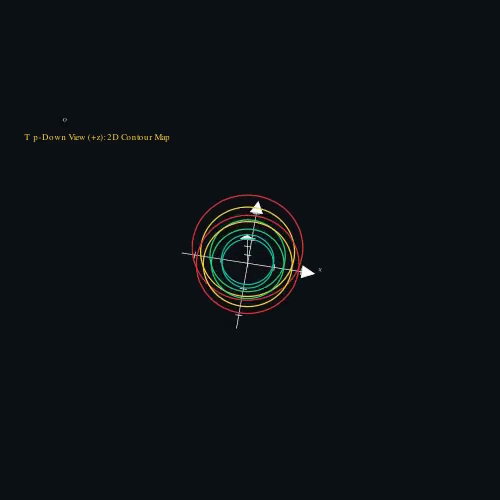
\includegraphics[width=0.92\linewidth, keepaspectratio]{TopDownLevelCurvesScene.png}
            
            \vspace{0.1cm}
            {\tiny \textcolor{gray}{\textit{Smooth transition: 3D Slicing $\longrightarrow$ Top-Down (+z) Contour Map}}}
        \end{column}
    \end{columns}
\end{frame}

\end{document}
